\documentclass[presentation,xcolor=pdftex,dvipsnames,table]{beamer}\usepackage[]{graphicx}\usepackage[]{color}
%% maxwidth is the original width if it is less than linewidth
%% otherwise use linewidth (to make sure the graphics do not exceed the margin)
\makeatletter
\def\maxwidth{ %
  \ifdim\Gin@nat@width>\linewidth
    \linewidth
  \else
    \Gin@nat@width
  \fi
}
\makeatother

\definecolor{fgcolor}{rgb}{0.345, 0.345, 0.345}
\newcommand{\hlnum}[1]{\textcolor[rgb]{0.686,0.059,0.569}{#1}}%
\newcommand{\hlstr}[1]{\textcolor[rgb]{0.192,0.494,0.8}{#1}}%
\newcommand{\hlcom}[1]{\textcolor[rgb]{0.678,0.584,0.686}{\textit{#1}}}%
\newcommand{\hlopt}[1]{\textcolor[rgb]{0,0,0}{#1}}%
\newcommand{\hlstd}[1]{\textcolor[rgb]{0.345,0.345,0.345}{#1}}%
\newcommand{\hlkwa}[1]{\textcolor[rgb]{0.161,0.373,0.58}{\textbf{#1}}}%
\newcommand{\hlkwb}[1]{\textcolor[rgb]{0.69,0.353,0.396}{#1}}%
\newcommand{\hlkwc}[1]{\textcolor[rgb]{0.333,0.667,0.333}{#1}}%
\newcommand{\hlkwd}[1]{\textcolor[rgb]{0.737,0.353,0.396}{\textbf{#1}}}%
\let\hlipl\hlkwb

\usepackage{framed}
\makeatletter
\newenvironment{kframe}{%
 \def\at@end@of@kframe{}%
 \ifinner\ifhmode%
  \def\at@end@of@kframe{\end{minipage}}%
  \begin{minipage}{\columnwidth}%
 \fi\fi%
 \def\FrameCommand##1{\hskip\@totalleftmargin \hskip-\fboxsep
 \colorbox{shadecolor}{##1}\hskip-\fboxsep
     % There is no \\@totalrightmargin, so:
     \hskip-\linewidth \hskip-\@totalleftmargin \hskip\columnwidth}%
 \MakeFramed {\advance\hsize-\width
   \@totalleftmargin\z@ \linewidth\hsize
   \@setminipage}}%
 {\par\unskip\endMakeFramed%
 \at@end@of@kframe}
\makeatother

\definecolor{shadecolor}{rgb}{.97, .97, .97}
\definecolor{messagecolor}{rgb}{0, 0, 0}
\definecolor{warningcolor}{rgb}{1, 0, 1}
\definecolor{errorcolor}{rgb}{1, 0, 0}
\newenvironment{knitrout}{}{} % an empty environment to be redefined in TeX

\usepackage{alltt}
\usetheme{Hannover}

\usepackage[utf8]{inputenc}
\usepackage[T1]{fontenc}
\usepackage[english, norsk]{babel}
\usepackage{xspace}
\usepackage{booktabs}
\usepackage{rotating}
\usepackage{graphicx}








\title[Degenerativ Nakke \\Troms�, UNN]{\textit{NKR - Degenerativ Nakke} \\
MÅNEDSRAPPORT \\
Troms�, UNN}
\date{}
\IfFileExists{upquote.sty}{\usepackage{upquote}}{}
\begin{document}
\begin{tiny}

\maketitle

\section{Registreringsoversikter}

\begin{frame}[fragile] {Innhold}
Dette er en sammenstilling av resultater  fra Norsk Kvalitetsregister for Ryggkirurgi, Degenerativ Nakke.
Alle registreringer er basert på registreringer i registeret per rapportdato. Data er hentet rett fra registeret og er ikke kvalitetssikret.
Datoer/årstall er basert på operasjonsdato. Resultatene som vises er i all hovedsak for de siste 12 måneder.
Tidsutvalg for rapportene er spesifisert for hver enkelt figur.

Rapporten viser følgende:
\begin{itemize}
\item  Antall registreringer per måned og avdeling.
\item	Registreringsoversikt med antall registreringer av hver type skjema.
\item	Figur, kvalind.
\item	Fig. kvalind
\end{itemize}

\end{frame}


\begin{frame}[fragile]
% latex table generated in R 3.4.1 by xtable 1.8-2 package
% Tue Mar 06 14:05:21 2018
\begin{table}[ht]
\centering
\begin{tabular}{lrrrrrrrrrrrrr}
  \hline
 & mar & apr & mai & jun & jul & aug & sep & okt & nov & des & jan & feb & Sum \\ 
  \hline
Aleris Helse AS & 0 & 1 & 3 & 2 & 1 & 1 & 0 & 3 & 1 & 0 & 0 & 0 & 12 \\ 
  Haukeland USH & 12 & 4 & 13 & 6 & 2 & 7 & 9 & 6 & 14 & 9 & 5 & 8 & 95 \\ 
  Oslo, RH & 39 & 25 & 36 & 37 & 6 & 23 & 28 & 20 & 27 & 13 & 3 & 0 & 257 \\ 
  Oslo, Ullevål USH & 28 & 16 & 13 & 12 & 6 & 10 & 6 & 17 & 20 & 13 & 3 & 0 & 144 \\ 
  Oslofjordklin., øst & 11 & 15 & 22 & 12 & 2 & 10 & 13 & 19 & 13 & 12 & 0 & 0 & 129 \\ 
  Oslofjordklinikken Vest & 7 & 2 & 5 & 3 & 5 & 1 & 5 & 4 & 7 & 0 & 0 & 0 & 39 \\ 
  Stavanger USH & 12 & 11 & 13 & 13 & 0 & 11 & 18 & 20 & 16 & 20 & 19 & 1 & 154 \\ 
  Tromsø, UNN & 6 & 5 & 7 & 8 & 1 & 3 & 2 & 6 & 7 & 2 & 5 & 1 & 53 \\ 
  Trondheim, St. Olav & 11 & 8 & 11 & 6 & 3 & 3 & 19 & 11 & 11 & 14 & 15 & 5 & 117 \\ 
  Volvat & 0 & 0 & 0 & 0 & 0 & 0 & 0 & 0 & 0 & 0 & 0 & 0 & 0 \\ 
  Sum & 126 & 87 & 123 & 99 & 26 & 69 & 100 & 106 & 116 & 83 & 50 & 15 & 1000 \\ 
   \hline
\end{tabular}
\caption{Antall registereringer (ferdigstilte legeskjema) per måned og avdeling, siste 12 måneder.} 
\end{table}

\end{frame}




\begin{frame}[fragile]
% latex table generated in R 3.4.1 by xtable 1.8-2 package
% Tue Mar 06 14:05:21 2018
\begin{table}[ht]
\centering
\begin{tabular}{lrrrrr}
  \hline
 & Lege & Pasient & Pasient (\%) & Oppfølging 3 mnd. & Oppfølging 3 mnd. (\%) \\ 
  \hline
Aleris Helse AS & 12 & 12 & 100.0 & 5 & 41.7 \\ 
  Haukeland USH & 95 & 93 & 97.9 & 47 & 49.5 \\ 
  Oslo, RH & 257 & 257 & 100.0 & 167 & 65.0 \\ 
  Oslo, Ullevål USH & 144 & 144 & 100.0 & 77 & 53.5 \\ 
  Oslofjordklin., øst & 129 & 129 & 100.0 & 70 & 54.3 \\ 
  Oslofjordklinikken Vest & 39 & 39 & 100.0 & 17 & 43.6 \\ 
  Stavanger USH & 154 & 154 & 100.0 & 57 & 37.0 \\ 
  Tromsø, UNN & 53 & 53 & 100.0 & 18 & 34.0 \\ 
  Trondheim, St. Olav & 117 & 117 & 100.0 & 42 & 35.9 \\ 
  Volvat & 0 & 0 &  & 0 &  \\ 
  Sum & 1000 & 998 & 99.8 & 500 & 50.0 \\ 
   \hline
\end{tabular}
\caption{Antall ferdigstilte skjema av hver type per måned og avdeling, siste 12 måneder.} 
\end{table}

\end{frame}






\section{Prosess}
\begin{frame}[fragile]
\begin{figure}[ht]
\centering
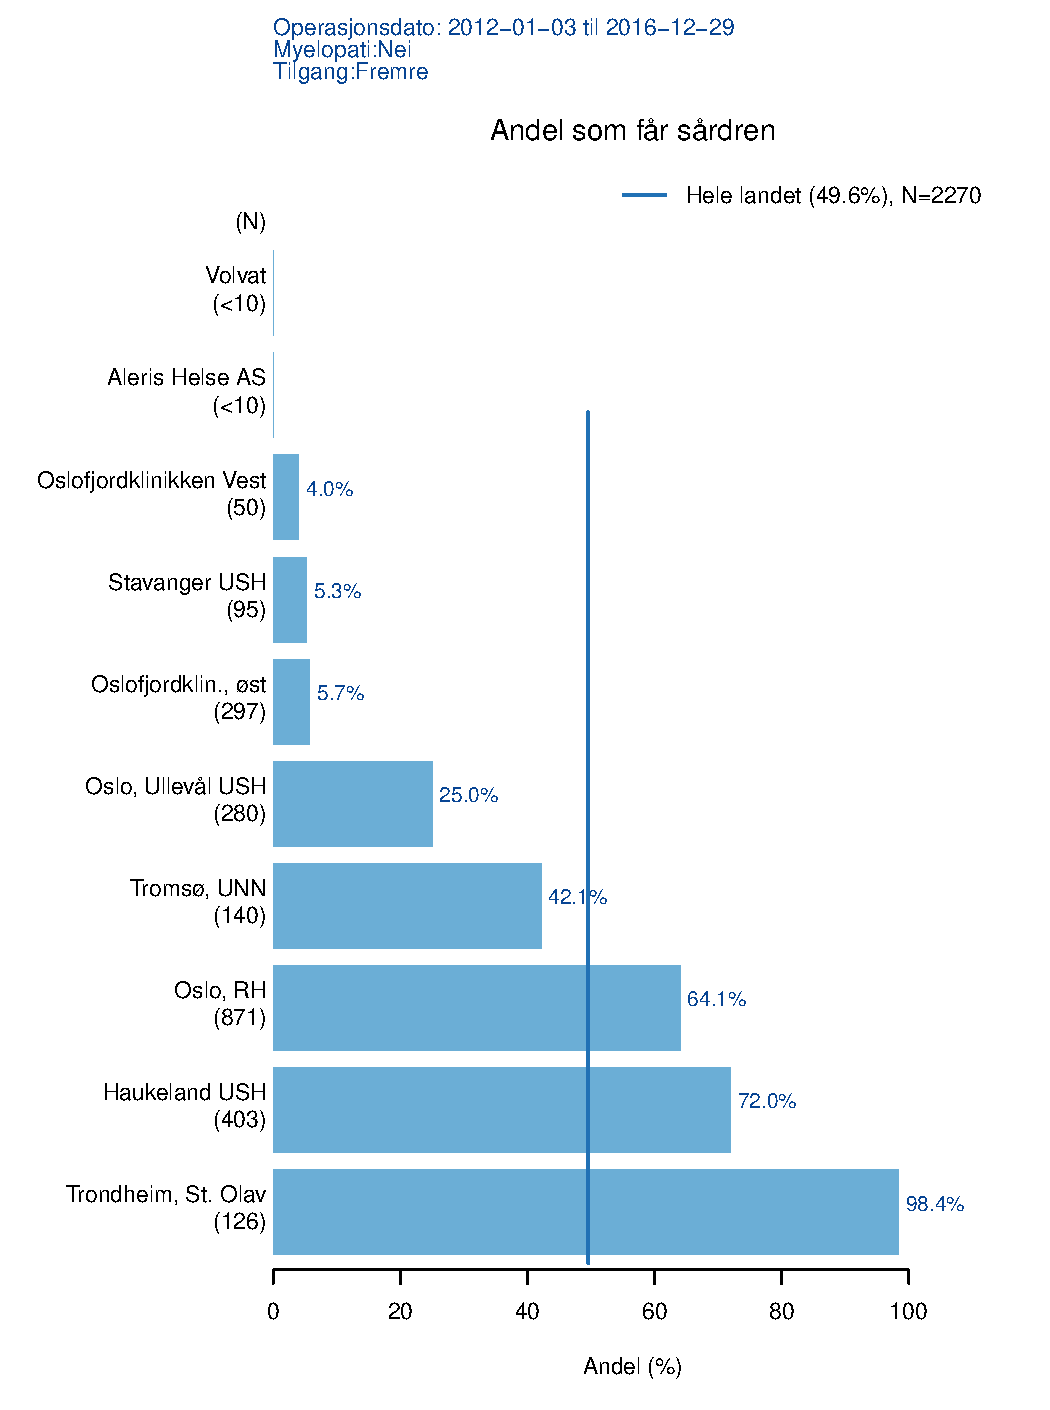
\includegraphics[scale=0.35]{NakkeSaardrenUmFSh.pdf}
\caption{Andel pasienter som har fått sårdren. }
\end{figure}

\section{Kvalitetsindikatorer}

\begin{frame}[fragile]
\begin{figure}[ht]
\centering
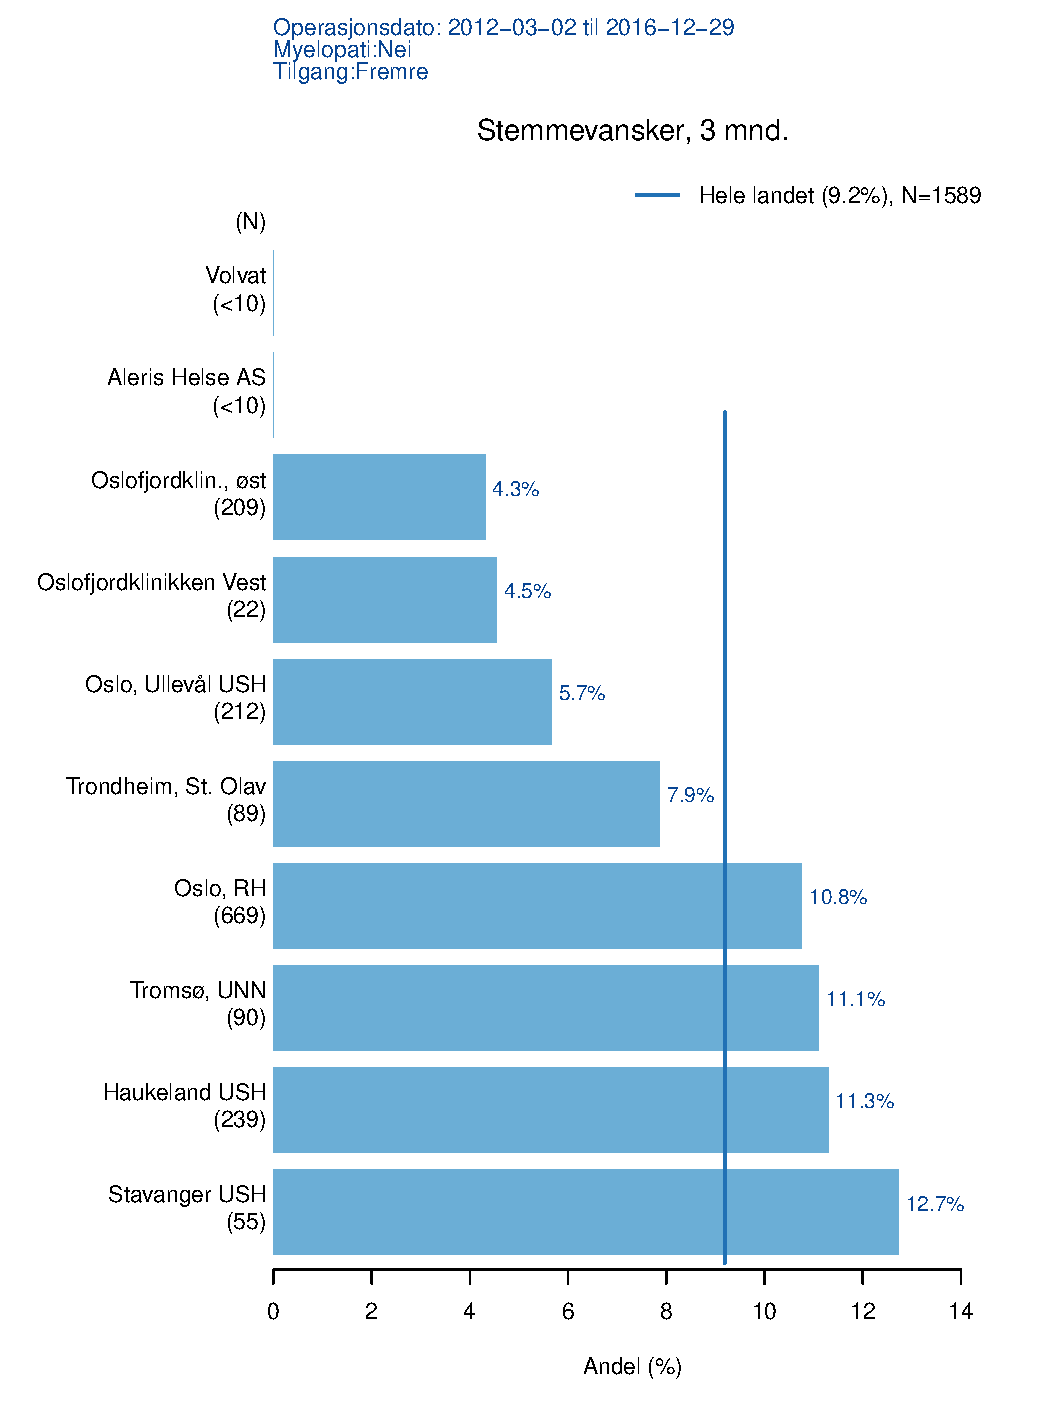
\includegraphics[scale=0.35]{NakkeStemme3mndSh.pdf.pdf}
\caption{Stemmevansker, 3 måneder etter operasjon. }
\end{figure}

\begin{frame}[fragile]
\begin{figure}[ht]
\centering
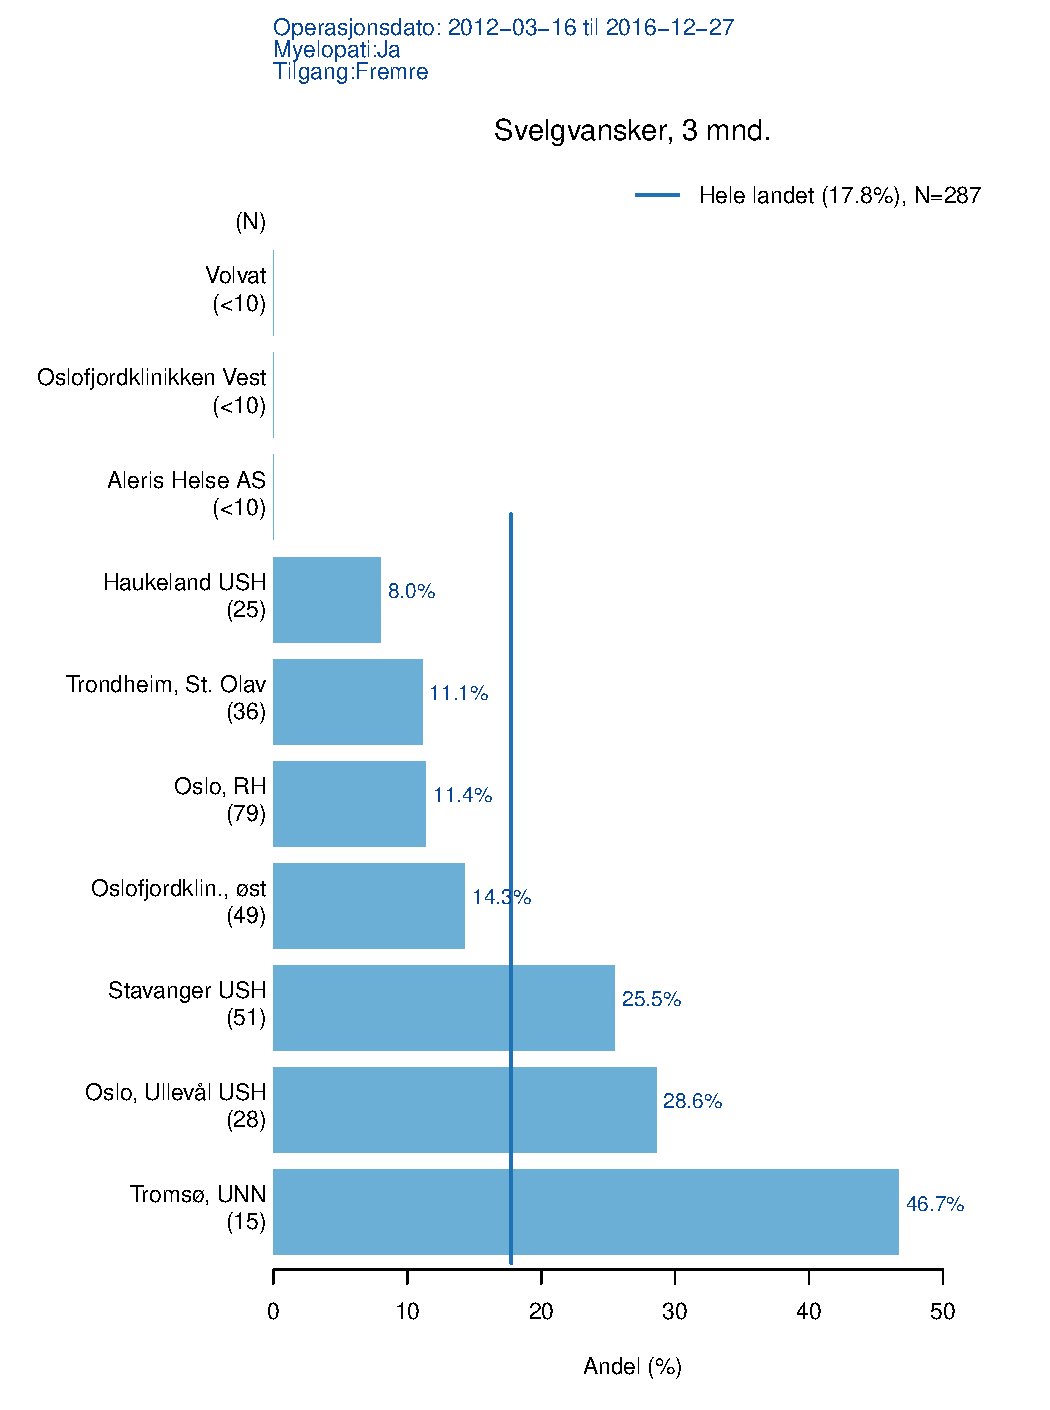
\includegraphics[scale=0.35]{NakkeSvelg3mndSh.pdf}
\caption{Svelgvansker, 3 måneder etter operasjon. }
\end{figure}


\begin{frame}[fragile]
\begin{figure}[ht]
\centering
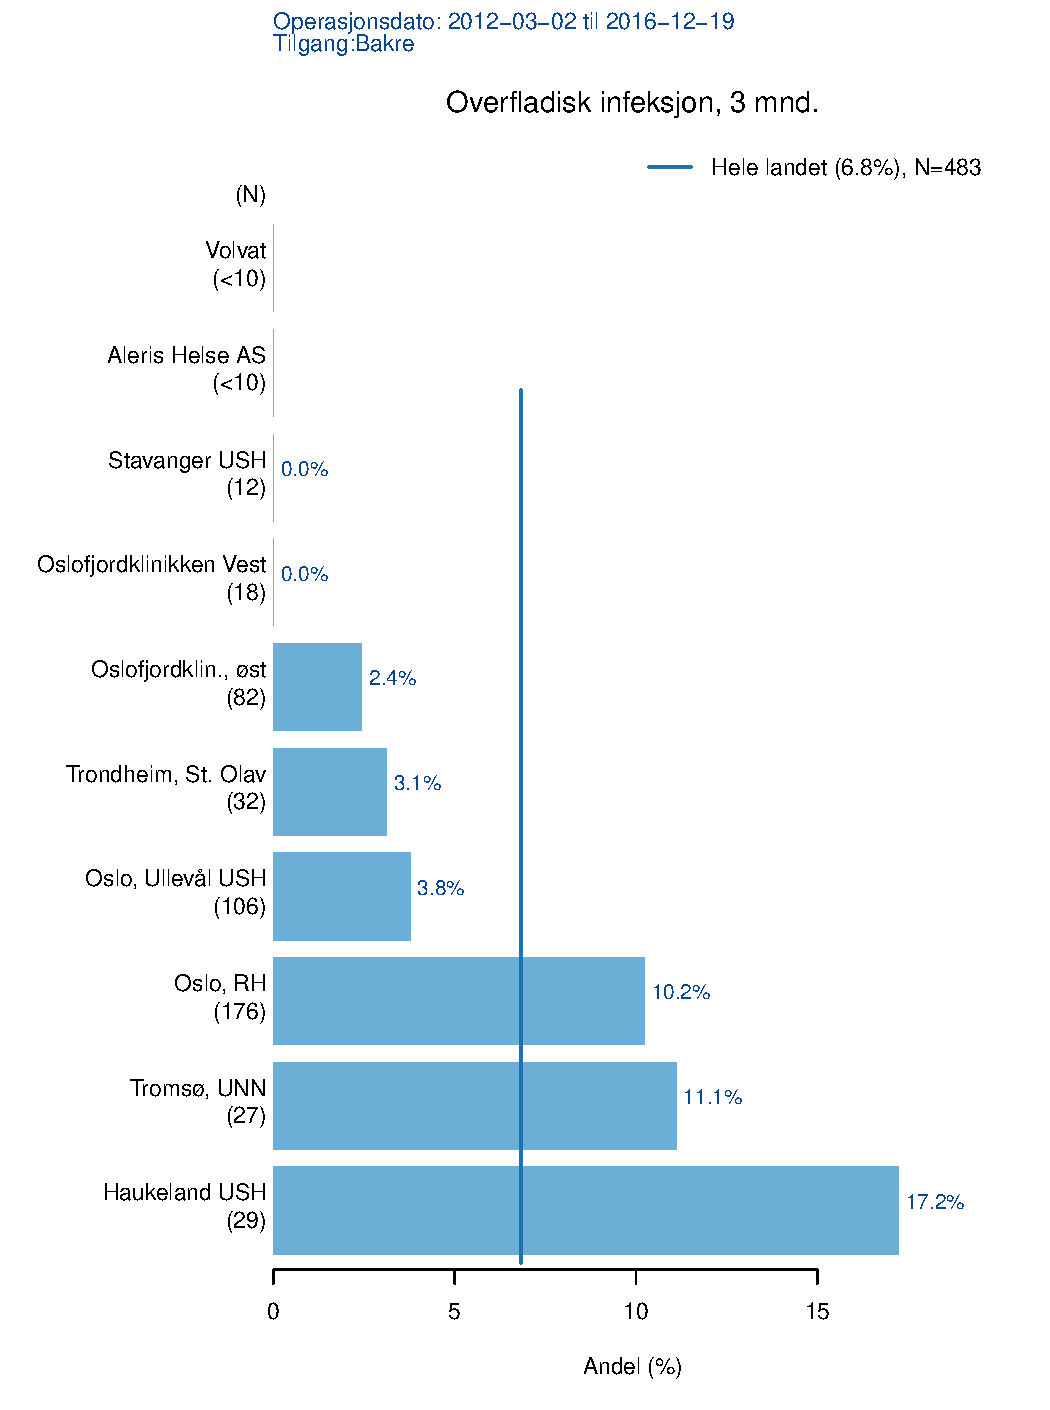
\includegraphics[scale=0.35]{NakkeKomplinfekOverfl3mndSh.pdf}
\caption{Overfladisk infeksjon, 3 måneder etter operasjon. }
\end{figure}

\begin{frame}[fragile]
\begin{figure}[ht]
\centering
\includegraphics[scale=0.35]{NakkeKomplinfek3mndSh.pdf}
\caption{Overfladisk infeksjon, 3 måneder etter operasjon. }
\end{figure}


\section{Pasientrapportert, 3 måneder}

\begin{frame}[fragile]
\begin{figure}[ht]
\centering
\includegraphics[scale=0.35]{NakkeFornoydBeh3mnd.pdf}
\caption{Registreringsforsinkelse. }
\end{figure}

begin{frame}[fragile]
\begin{figure}[ht]
\centering
\includegraphics[scale=0.35]{NakkeNytteOpr3mndSh.pdf}
\caption{Registreringsforsinkelse. }
\end{figure}


\end{frame}


\end{tiny}
\end{document}
